\documentclass[twoside, 12pt]{epstfg}


\usepackage{lipsum}
\usepackage[numbers]{natbib}
\usepackage{fancysprefs}
\usepackage{booktabs}
\usepackage{wrapfig}
\usepackage{enumitem}
\usepackage{xfrac}
\usepackage{multirow}
\usepackage{tikz}

%\usetikzlibrary{arrows}
%\usetikzlibrary{patterns}
%\usetikzlibrary{intersections}
%\usetikzlibrary{calc}
%\usetikzlibrary{fadings}

%\definecolor{palette1}{HTML}{1B9E77}
%\definecolor{palette2}{HTML}{D95F02}
%\definecolor{palette3}{HTML}{7570B3}
%\definecolor{palette4}{HTML}{E7298A}
%\definecolor{palette5}{HTML}{66A61E}
%\definecolor{palette6}{HTML}{E6AB02}
%\definecolor{palette7}{HTML}{A6761D}
%\definecolor{palette8}{HTML}{666666}

\tikzstyle{IpNode}=[rectangle, draw=black, thick, inner sep=12pt]
\tikzstyle{NewIpNode}=[IpNode, fill=green]
\tikzstyle{MacNode}=[circle, draw=black, thick, inner sep=7pt]
\tikzstyle{NewMacNode}=[MacNode, fill=green]

\tikzstyle{OpenEdge}=[->, ultra thick]
\tikzstyle{CloseEdge}=[OpenEdge, red]
\tikzstyle{VirtualEdge}=[CloseEdge, double]
\tikzstyle{NewOpenEdge}=[OpenEdge, densely dashed]
\tikzstyle{NewCloseEdge}=[CloseEdge, densely dashed]
\tikzstyle{NewVirtualEdge}=[VirtualEdge, densely dashed]
\tikzset{>=latex}

\bibliographystyle{abbrv}

\title[spa]{Reconstrucción de caminos y deteción de dispositivos}
\title[eng]{Path reconstruction}
\author{David Moreno Maldonado}
\tutor{Guillermo Julián Moreno}
\date[spa]{Mayo 2020}
\date[eng]{May 2020}
\group[spa]{Naudit}
\group[eng]{Naudit}
\department[spa]{Tecnología Electrónica y de las comunicaciones}
\department[eng]{Department}

\setdegreeDouble

%Resumen
%Abstract (resumen en ingles)

%Glosario

\begin{document}

\selectlanguage{spanish}

\frontmatter

\maketitle[spa]
% \maketitle[eng]

\makeinnertitle[spa]
% \makeinnertitle[eng]

%\makeabstract[spa]
%\makeabstract[eng]

\tableofcontents
\clearpage
\listoftables
\clearpage
\listoffigures
\cleardoublepage

\printnoidxglossaries

\mainmatter

\chapter{Introducción y motivación}

\section{Motivación}

\section{Objetivos}

\section{Estructura del documento}


\chapter{Estado del arte}
A lo largo de este capítulo se expondrán diferentes herramientas actuales que se utilizan para el análisis de redes con especial atención al análisis de flujos IP, así como métodos para la detección de distintos tipos de dispositivos.

\section{Herramientas de análisis de redes pasivas}
El análisis de redes desde el punto de vista de la reconstrucción del flujo IP de los paquetes y la detección de dispositivos intermedios de una manera pasiva se basa en la utilización de trazas pcap ya capturadas. Estas se abren con diferentes programas que nos aportan información relevante sobre los paquetes y los hosts que se conectan. Se presentan ahora algunas de las más populares y más interesantes que se han encontrado \cite{Gandhi2014} \cite{bestNetAna}

\subsection{Wireshark}
\subsection{Netflow}
\subsection{Capsa}
\subsection{Etherape}
\subsection{GlassWire}

\section{Herramientas de análisis de redes activas}
Aunque no es muy relevante para la realización de este trabajo, cabe mencionar que existen maneras de analizar redes de una manera activa. Esto es especialmente útil para la reconstrucción de los caminos y la detección de dispositivos. Obviamente, esto será mucho más intrusivo que el análisis pasivo, pero se tiene un mayor control de los datos obtenidos y el procesado posterior es menor. Algunos ejemplos son los siguientes.

\subsection{OpenFlow (protocolo)}

\section{Métodos de detección de dispositivos}
%Esta seccion variara en funcion de los dispositivos que se detecten finalmente
\subsection{Detección de routers NAT}
\cite{Krmicek}
\subsection{Detección de firewalls}
\subsection{Detección de balanceadores de carga}

\section{Conclusiones del capítulo}

\chapter{Análisis del problema}
\label{chap:Analisis}
A lo largo de este capítulo se expondrán los dos grandes problemas que se abordan durante la implementación del programa, así como el razonamiento que se siguió para hallar sus soluciones. El primero de ellos es la reconstrucción de caminos basándonos en la información que nos llega paquete a paquete. Se exponen unos cuantos casos básicos y otros de ejemplo para una mayor comprensión. El segundo es el de detectar los diferentes dispositivos en la red una vez que ya se han reconstruido los caminos ...

\section{Reconstrucción de caminos}
%Especificar mejor que no se presupone que los paquetes son recibidos en orden salvo cuando no hay mas remedio
%Relacionar tambien los casos como grafo en general con los que no nos encontraremos nunca por como son las redes
El primer problema que afrontamos es el de inferir el camino que realizan los paquetes de un determinado flujo IP en base a la observación de los saltos individuales. Dada la naturaleza de una red en concreto este proceso puede ser complicado debido a la existencia de dispositivos intermedios (que más adelante pretendemos detectar) o bifurcaciones en los caminos que llevan de una IP a otra. Esto se puede dar por la caida temporal de enlaces entre nodos de la red o simplemente por las características de la red en sí.

\subsection{Planteamiento del problema y caso inicial}
Para poder plantearnos una solución, tenemos primero que establecer las bases del problema. Dadas dos nodos IPs (IPA e IPB) tenemos una visión parcial o total de los saltos que se hacen entre estos dos nodos y que les permiten comunicarse. En general, la información que recibiremos será con la forma de un paquete estandar, es decir, con una IP origen, MAC origen, MAC destino e IP destino. Vamos a recurrir a grafos para visualizar mejor el problema y enfocar la resolución del camino. Dado un par de IPs podemos expresar el flujo de información que hay entre ellas mediante un grafo unidireccional. Cada IP y cada MAC se representan como un nodo (rectangulares y circulares, respectivamente) y las aristas orientadas representan la conexión entre dos nodos. Diferenciamos, además, entre dos tipos de aristas: las cerradas (en rojo), entre las que ya no se podrán insertar más nodos, y las abiertas (en negro), entre las que aún se pueden insertar más nodos. En realidad, para cada flujo en específico no nos es importante la IP origen e IP destino, ya que al estar reconstruyendo flujos IP estas van a ser constantes. Por lo tanto, sin perdida de generalidad, podemos asumir que en cada paquete la información que nos interesa es la de MAC origen y MAC destino, y a partir de ahí razonaremos que nodos y aristas se deben de insertar en el grafo. 

Una vez que vemos el primer paquete entre IPA e IPB con una MAC origen (MAC1) y una MAC destino (MAC2) asumimos que ese salto existe físicamente y que no puede existir ningún otro salto intermedio, ya que dado el caso lo habríamos visto. Marcamos ese salto como cerrado. De esta manera, cada vez que veamos un nuevo salto entre IPA e IPB expandirá el flujo en cualquiera de las dos aristas restantes con nuevos nodos, pero estos nunca se interpondrán entre MAC1 y MAC2. Este caso queda representado en el grafo de la \fref{fig:Analisis:BasicFlow}

\begin{figure}
\centering
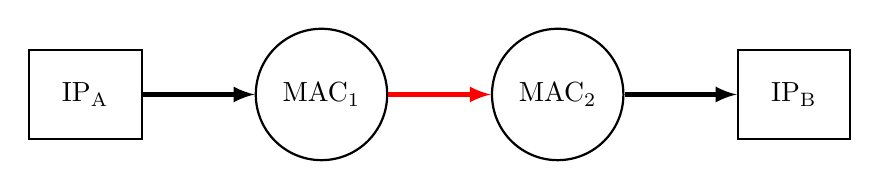
\begin{tikzpicture}
\node[IpNode](IPA) at (0,0) {IP\textsubscript{A}};
\node[MacNode](MAC1) at (3,0) {MAC\textsubscript{1}};
\node[MacNode](MAC2) at (6,0) {MAC\textsubscript{2}};
\node[IpNode](IPB) at (9,0) {IP\textsubscript{B}};

\draw[OpenEdge](IPA) -- (MAC1);
\draw[CloseEdge](MAC1) -- (MAC2);
\draw[OpenEdge](MAC2) -- (IPB);

\end{tikzpicture}
\caption[Flujo básico entre dos IPs]{Flujo básico entre IPA e IPB}
\label{fig:Analisis:BasicFlow}
\end{figure}

Este escenario nos deja con varias posibilidades que tenemos que tener en cuenta de manera especial: inserciones estándar de nuevos nodos, bifurcaciones y caminos huérfanos. De aquí en adelante se supondrá siempre el grafo en la situación de \fref{fig:Analisis:BasicFlow} como situación inicial. Decidiremos el caso en el que nos encontramos según la relación de las MACs origen y destino del nuevo paquete con las MACs ya introducidas en el grafo.

\subsection{Inserción estándar}
Con una inserción estándar nos referimos al caso en el que simplemente estamos añadiendo información al grafo en alguna de las aristas abiertas. Este es el caso en el que el nuevo paquete cumple una de estas dos condiciones:
\begin{itemize}
    \item La MAC origen coincide con la última MAC del grafo. Suponiendo la situación inicial y la llegada de un paquete con MAC origen igual a MAC2 y MAC destino igual a MAC3 el resultado es el del grafo de la \fref{fig:Analisis:AddingLast}.
    \item La MAC destino coincide con la primera MAC del grafo. Suponiendo la situación inicial y la llegada de un paquete con MAC origen igual a MAC0 y MAC destino igual a MAC1 el resultado es el del grafo de la \fref{fig:Analisis:AddingFirst}.
\end{itemize}

\begin{figure}
\centering
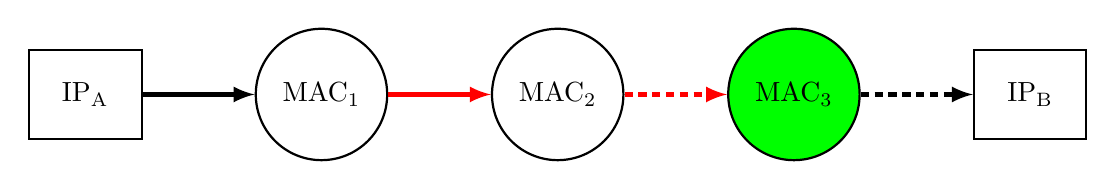
\begin{tikzpicture}
\node[IpNode](IPA) at (0,0) {IP\textsubscript{A}};
\node[MacNode](MAC1) at (3,0) {MAC\textsubscript{1}};
\node[MacNode](MAC2) at (6,0) {MAC\textsubscript{2}};
\node[NewMacNode](MAC3) at (9,0) {MAC\textsubscript{3}};
\node[IpNode](IPB) at (12,0) {IP\textsubscript{B}};

\draw[OpenEdge](IPA) -- (MAC1);
\draw[CloseEdge](MAC1) -- (MAC2);
\draw[NewCloseEdge](MAC2) -- (MAC3);
\draw[NewOpenEdge](MAC3) -- (IPB);
\end{tikzpicture}
\caption[Ejemplo inserción básica 1]{Añadimos una nueva MAC al final del flujo}
\label{fig:Analisis:AddingLast}
\end{figure}

\begin{figure}
\centering
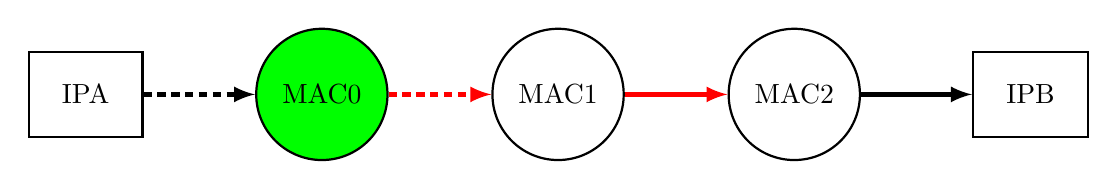
\begin{tikzpicture}
\node[IpNode](IPA) at (0,0) {IPA};
\node[NewMacNode](MAC0) at (3,0) {MAC0};
\node[MacNode](MAC1) at (6,0) {MAC1};
\node[MacNode](MAC2) at (9,0) {MAC2};
\node[IpNode](IPB) at (12,0) {IPB};

\draw[NewOpenEdge](IPA) -- (MAC0);
\draw[NewCloseEdge](MAC0) -- (MAC1);
\draw[CloseEdge](MAC1) -- (MAC2);
\draw[OpenEdge](MAC2) -- (IPB);
\end{tikzpicture}
\caption[Ejemplo inserción básica 2]{Añadimos una nueva MAC al comienzo del flujo}
\label{fig:Analisis:AddingFirst}
\end{figure}

En ambos casos únicamente se añade información de un nodo y se cierra la arista correspondiente al salto físico que hemos visto. Utilizando esta operación de inserción básica podemos seguir añadiendo nodos MAC al flujo indefinidamente.

\subsection{Bifurcación}
En el caso de que alguna de las dos MAC del nuevo paquete se encuentre ya en nuestro grafo, pero no nos hallemos en ninguno de los casos anteriores tenemos una bifurcación. De esta manera, el nuevo nodo se insertará entre el nodo que ya está en el grafo y la IP correspondiente. A continuación se muestran un par de ejemplos de bifurcaciones en base al estado inicial en los grafos de la \fref{fig:Analisis:Bifurcation1} y de la \fref{fig:Analisis:Bifurcation2}.

\begin{figure}
\centering
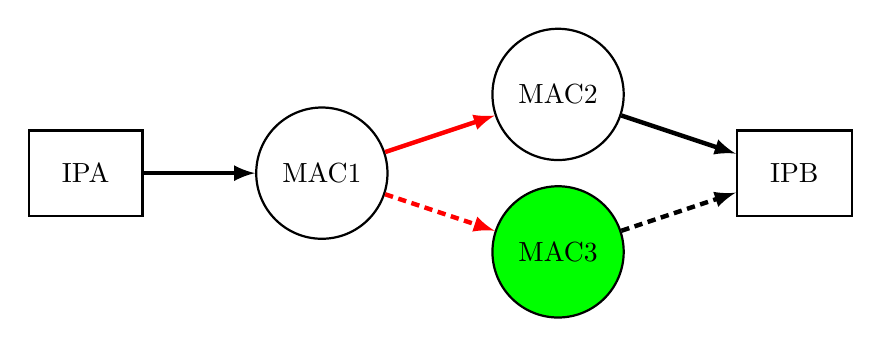
\begin{tikzpicture}
\node[IpNode](IPA) at (0,1) {IPA};
\node[MacNode](MAC1) at (3,1) {MAC1};
\node[MacNode](MAC2) at (6,2) {MAC2};
\node[NewMacNode](MAC3) at (6,0) {MAC3};
\node[IpNode](IPB) at (9,1) {IPB};

\draw[OpenEdge](IPA) -- (MAC1);
\draw[CloseEdge](MAC1) -- (MAC2);
\draw[NewCloseEdge](MAC1) -- (MAC3);
\draw[NewOpenEdge](MAC3) -- (IPB);
\draw[OpenEdge](MAC2) -- (IPB);
\end{tikzpicture}
\caption[Ejemplo de bifurcación 1]{Bifurcación al añadir paquete con MAC origen igual a MAC1 y MAC destino igual a MAC3}
\label{fig:Analisis:Bifurcation1}
\end{figure}

\begin{figure}
\centering
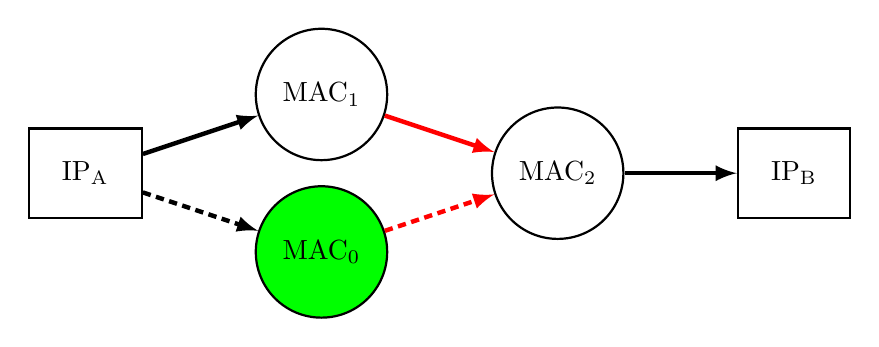
\begin{tikzpicture}
\node[IpNode](IPA) at (0,1) {IP\textsubscript{A}};
\node[NewMacNode](MAC0) at (3,0) {MAC\textsubscript{0}};
\node[MacNode](MAC1) at (3,2) {MAC\textsubscript{1}};
\node[MacNode](MAC2) at (6,1) {MAC\textsubscript{2}};
\node[IpNode](IPB) at (9,1) {IP\textsubscript{B}};

\draw[NewOpenEdge](IPA) -- (MAC0);
\draw[OpenEdge](IPA) -- (MAC1);
\draw[CloseEdge](MAC1) -- (MAC2);
\draw[NewCloseEdge](MAC0) -- (MAC2);
\draw[OpenEdge](MAC2) -- (IPB);
\end{tikzpicture}
\caption[Ejemplo de bifurcación 2]{Bifurcación al añadir paquete con MAC origen igual a MAC0 y MAC destino igual a MAC2}
\label{fig:Analisis:Bifurcation2}
\end{figure}

Utilizando las dos maneras de insertar que se han descrito hasta el momento se puede llegar a cualquier grafo de los que describen un flujo entre dos IPs relacionado con MACs. Se propone un ejemplo en base al estado inicial añadiendo unos cuantos paquetes y observando como avanza el grafo. Se puede observar en la \fref{fig:Analisis:ComplexFlow}.%Que grafos podemos tener en la realidad???

\begin{figure}
\centering
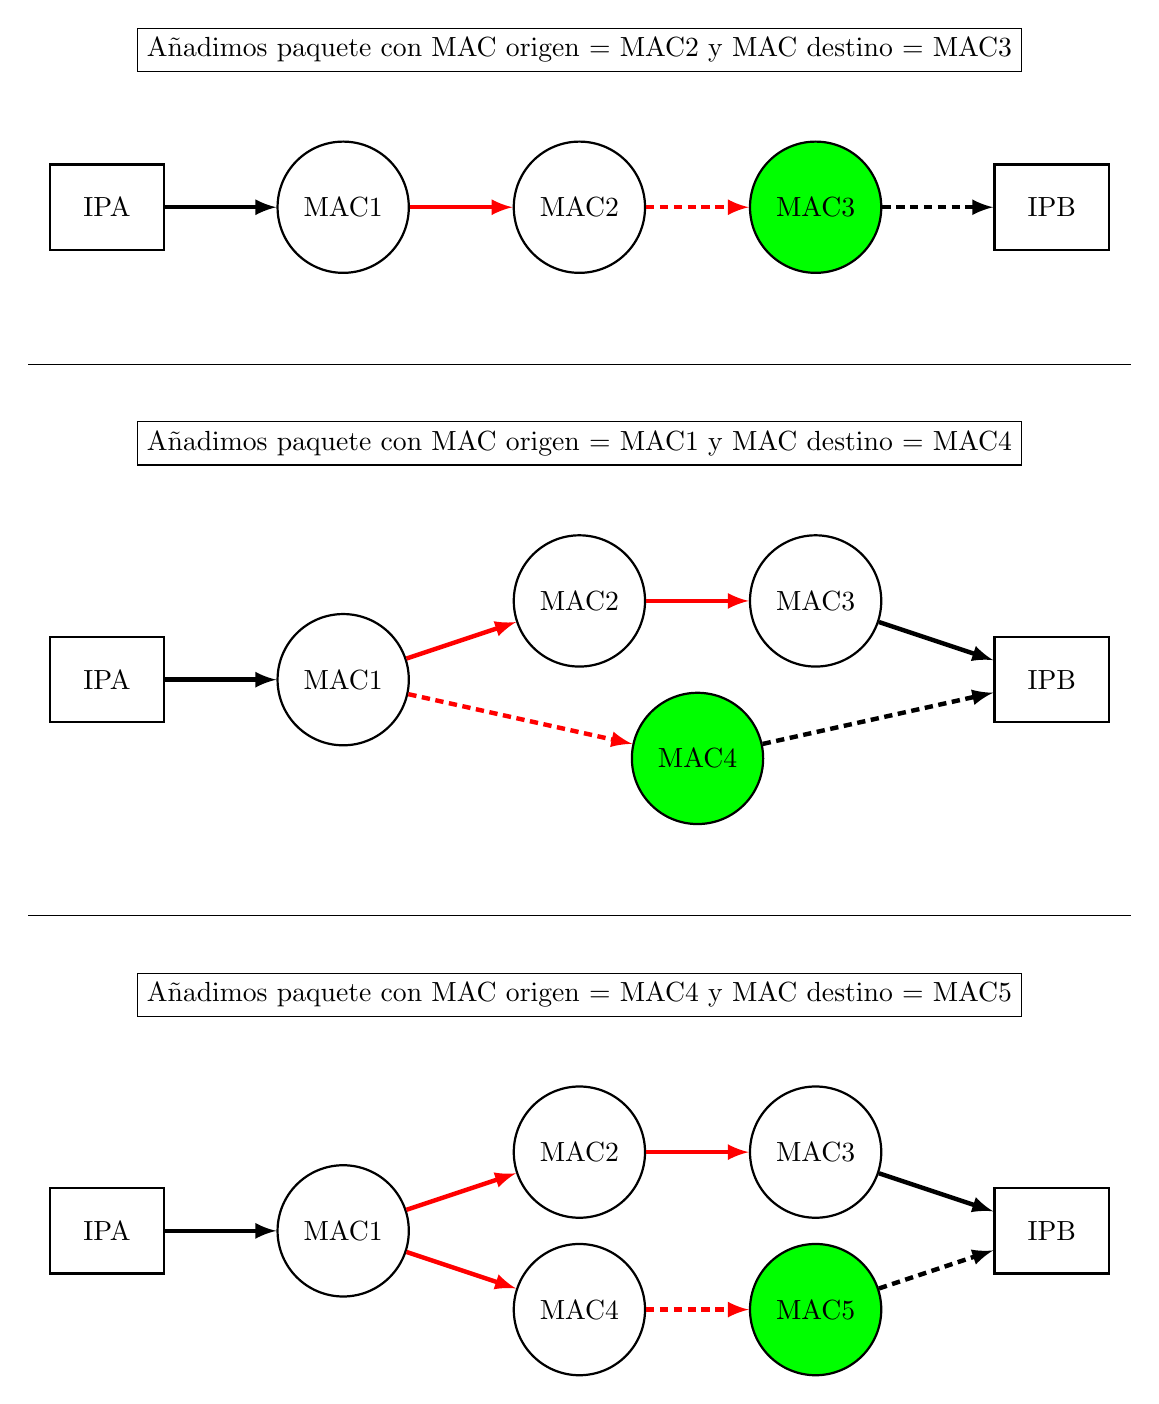
\begin{tikzpicture}
\node[draw] at (6,0) {Añadimos paquete con MAC origen = MAC2 y MAC destino = MAC3};

\node[IpNode](1IPA) at (0,-2) {IPA};
\node[MacNode](1MAC1) at (3,-2) {MAC1};
\node[MacNode](1MAC2) at (6,-2) {MAC2};
\node[NewMacNode](1MAC3) at (9,-2) {MAC3};
\node[IpNode](1IPB) at (12,-2) {IPB};

\draw[OpenEdge](1IPA) -- (1MAC1);
\draw[CloseEdge](1MAC1) -- (1MAC2);
\draw[NewCloseEdge](1MAC2) -- (1MAC3);
\draw[NewOpenEdge](1MAC3) -- (1IPB);

\draw (-1,-4) -- (13,-4);

%%%%%%%%%%%%%%%%%%%%%%%%%%%%%%%%%%%%%%%%%

\node[draw] at (6,-5) {Añadimos paquete con MAC origen = MAC1 y MAC destino = MAC4};

\node[IpNode](2IPA) at (0,-8) {IPA};
\node[MacNode](2MAC1) at (3,-8) {MAC1};
\node[MacNode](2MAC2) at (6,-7) {MAC2};
\node[NewMacNode](2MAC4) at (7.5,-9) {MAC4};
\node[MacNode](2MAC3) at (9,-7) {MAC3};
\node[IpNode](2IPB) at (12,-8) {IPB};

\draw[OpenEdge](2IPA) -- (2MAC1);
\draw[CloseEdge](2MAC1) -- (2MAC2);
\draw[NewCloseEdge](2MAC1) -- (2MAC4);
\draw[CloseEdge](2MAC2) -- (2MAC3);
\draw[OpenEdge](2MAC3) -- (2IPB);
\draw[NewOpenEdge](2MAC4) -- (2IPB);

\draw (-1,-11) -- (13,-11);

%%%%%%%%%%%%%%%%%%%%%%%%%%%%%%%%%%%%%%%%%%%%%%

\node[draw] at (6, -12) {Añadimos paquete con MAC origen = MAC4 y MAC destino = MAC5};

\node[IpNode](3IPA) at (0,-15) {IPA};
\node[MacNode](3MAC1) at (3,-15) {MAC1};
\node[MacNode](3MAC2) at (6,-14) {MAC2};
\node[MacNode](3MAC4) at (6,-16) {MAC4};
\node[MacNode](3MAC3) at (9,-14) {MAC3};
\node[NewMacNode](3MAC5) at (9,-16) {MAC5};
\node[IpNode](3IPB) at (12,-15) {IPB};

\draw[OpenEdge](3IPA) -- (3MAC1);
\draw[CloseEdge](3MAC1) -- (3MAC2);
\draw[CloseEdge](3MAC1) -- (3MAC4);
\draw[CloseEdge](3MAC2) -- (3MAC3);
\draw[NewCloseEdge](3MAC4) -- (3MAC5);
\draw[OpenEdge](3MAC3) -- (3IPB);
\draw[NewOpenEdge](3MAC5) -- (3IPB);
\end{tikzpicture}
\caption[Ejemplo de superflujo compuesto]{Evolución del grafo tras añadir diferentes paquetes.}
\label{fig:Analisis:ComplexFlow}
\end{figure}

\newpage
\subsection{Camino huérfano}

Existe un caso particular en el que hay que prestar especial atención, los caminos huérfanos. Esta situación se da cuando el paquete que analizamos no tiene ninguna MAC incluida en el grafo. LLegados a este punto no tenemos manera de saber en que lugar colocar la nueva información que se nos da si no asumimos alguna condición más o extraemos más información del paquete. Es aquí donde entran en juego los atributos de orden que nos servirán para, dados dos nodos, saber cual se encuentra antes o después en el grafo y así poder insertarlo. El procedimiento será intentar ordenar la MAC origen del nuevo paquete ya que la MAC destino tiene una relación física directa con el otro e irá justo después; lo que en nuestro grafo se traduciría en una arista cerrada entre los nuevos nodos. En el caso de que el paquete nuevo no pueda ser ordenado podemos proceder de dos maneras: guardar la información del paquete para volver a intentar insertarlo en un futuro cuando existan más nodos en el grafo o descartarlo, perdiendo así la información.

El atributo de orden que vamos a utilizar es el TTL de los paquetes. Es claro ver que, dados dos paquetes, si uno tiene un TTL menor que otro podemos determinar que el primer enlace está antes en el flujo IP. Supongámos que nos encontramos en el estado inicial del grafo de la \fref{fig:Analisis:BasicFlow}, si tenemos información de que los nodos de MAC1 y MAC2 tenían un TTL=64 y nos llega un paquete con MAC origen = MAC3, MAC destino = MAC4 y TTL=63. Como ya hemos dicho, no tenemos una manera de introducir su información en el grafo, pero utilizando la información del TTL sabemos que este paquete está situado después de lo que ya teníamos. El estado del grafo quedaría como se oberva en la \fref{fig:Analisis:OrphanPath}. Cabe resaltar que la  arista entre MAC2 y MAC3 queda cerrada, pero es una arista especial en cuanto a que hemos inferido el salto entre MAC2 y MAC3 gracias a la información del TTL, es por esto que la marcaremos como arista virtual (arista con doble linea). Esto tendrá su utilidad a la hora de detectar dispositivos.

\begin{figure}
\centering
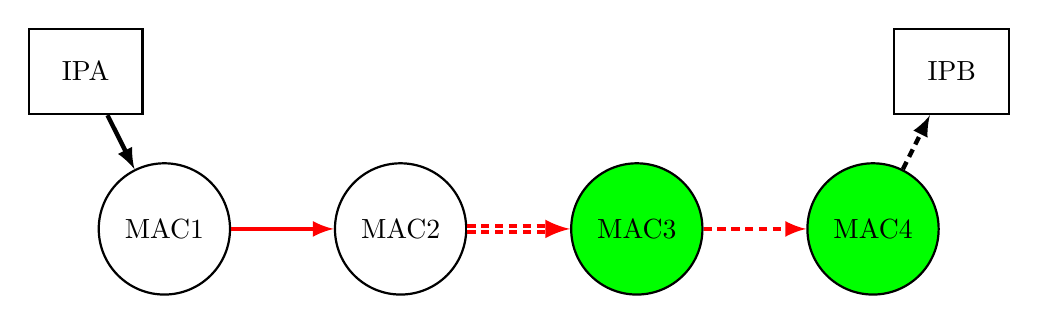
\begin{tikzpicture}
\node[IpNode](IPA) at (0,0) {IPA};
\node[MacNode](MAC1) at (1,-2) {MAC1};
\node[MacNode](MAC2) at (4,-2) {MAC2};
\node[NewMacNode](MAC3) at (7,-2) {MAC3};
\node[NewMacNode](MAC4) at (10,-2) {MAC4};
\node[IpNode](IPB) at (11,0) {IPB};

\draw[OpenEdge](IPA) -- (MAC1);
\draw[CloseEdge](MAC1) -- (MAC2);
\draw[NewVirtualEdge](MAC2) -- (MAC3);
\draw[NewCloseEdge](MAC3) -- (MAC4);
\draw[NewOpenEdge](MAC4) -- (IPB);
\end{tikzpicture}
\caption[Ejemplo de resolución de camino huérfano]{Insetamos el paquete huérfano gracias a la información del TTL.}
\label{fig:Analisis:OrphanPath}
\end{figure}

\subsection{Problemas con el orden de los paquetes.}

\subsection{Relación entre el número de nodos y el número de aristas}
%Indicar mas formalmente como y por que hemos estimado que las bifurcaciones siguen una distribución de Poisson y hemos estimado lambda por maxima verosimilitud (media poblacional con respecto a varias trazas). Posiblemente esto vaya en un anexo y haya que referenciar algun libro de texto
A la hora de la implementación, como se verá más adelante, tendrá utilidad el conocer cual es la relación entre la cantidad de nodos y la cantidad de aristas que tiene nuestro grafo. La notación que seguiremos en este apartado sera la siguiente:
\begin{align*}
	n =& \mathbin{\#}\{\textit{nodos en un grafo}\} \\
	a =& \mathbin{\#}\{\textit{aristas en un grafo}\} \\
	b =& \mathbin{\#}\{\textit{bifurcaciones en un grafo}\}
\end{align*}
Es claro ver que para un grafo sin bifurcaciones \(a = n-1\), ya que todo nodo estará unido con el siguiente por una arista salvo el último. Por cada bifurcación, añadiremos al grafo un nodo y dos aristas, la que bifurca el nuevo camino y la que lo vuelve a unir, es decir, estamos añadiendo una arista de más. Nos es indiferente cuanto de largo sea el camino de una bifurcación ya que siempre se mantendrá la relación de que añadimos una arista por cada nodo. En conclusión, podemos afirmar que la relación entre el número de aristas y nodos es:
\begin{equation*}
    a = (n - 1) + b
\end{equation*}
El número de bifurcaciones es uan variable aleatoria que depende de las características de cada red en específico, pero podemos ver que sigue una distribución de Poisson. De esta manera, podemos calcular el número de aristas que esperamos ver en función de los nodos. 
\begin{align*}
 \mathbb{E}(a) =&\ (n - 1) + \mathbb{E}(\bb Poisson(\lambda))\\
 \mathbb{E}(a) =&\ (n - 1) + \lambda
\end{align*}
Para poder calcular el número de aritas necesitamos saber cuanto vale el parámetro $\lambda$, pero este valor no es general y debemos estimarlo. El procedimiento para estimarlo es por máxima verosimilitud. Calculamos $\lambda = \widehat{\lambda} = \bar{b}$, siendo $\bar{b}$ la media muestral de bifurcaciones en función de los nodos que hay en un flujo. Hay que tener en cuenta que, por las características de los grafos que utilizamos, los nodos IP no pueden tener bifurcaciones. Los resultados de las medidas son $\bar{b} = 0,0034$. Vemos que el número de bifurcaciones es muy bajo, pudiendo tomar como resultado final $\mathbb{E}(a) \approx n - 1$ sobre todo teniendo en cuenta que el número de nodos en total será grande.

\section{Identificación de elementos en el superflujo}

\chapter{Estructura y desarrollo}
\label{chap:Desarrollo}
\section{Decisiones generales de desarrollo}
La primera parte del desarrollo consistió en implementar la parte de reconstrucción de caminos. Esto se realizó como parte de un programa más amplio llamado fisher, programa escrito en C. La decisión de utilizar este lenguaje es por las características del proyecto, ya que se analizarán archivos de un gran tamaño. Lo que nos permite C es gestionar la memoria a un nivel más bajo, con lo que podemos realizar los mismos procesos que con otros lenguajes de más alto nivel, pero con una mayor eficiencia. Ya en la descripción de la motivación del proyecto se mencionó que uno de los problemas que se encontró en el anterior intento de desarrollar un programa similar en Python fue la lentitud del mismo. Se pretende que con este cambio en el lenguaje de desarrollo se lleguen a las velocidades esperadas en el análisis así como a una mayor eficiencia en memoria.

El análisis de tráfico forma parte de un programa más grande llamado fisher. Dicha aplicación se centraba en el análisis de trazas pcap mediante la definición de funciones que se encargan de la inicialización, preprocesado, análisis, postprocesado y salida de los registros de la traza pcap. Se disponen de diferentes lectores de trazas (NDLeeTrazas, lpcap, mmpcap y hpcap), en general se usará NDLeeTrazas por defecto. Se han utilizado y modificado varias de las librerias de este programa, haciendose uso de facilidades como el log, utilidades para estructuras ip y mac, el gestor de memoria para generar pools de memoria o la estructura de tests ya desarrollada para garantizar la funcionalidad del código escrito.

En un comienzo se pensó que con el análisis de trazas pcap sería suficiente. Sin embargo, se consideró que sería útil que fuera posible realizar el análisis de superflujos a partir de otros ficheros de origen. No siempre se iba a disponer de la traza pcap en bruto y la librería tiene la flexibilidad suficiente para adaptarse a diferentes tipos de entrada que le aporten más o menos información. El ejemplo más claro fue el de la salida de 'Procesa' un programa que lee y extrae información del tráfico de red y la presenta como registros por flujo. El programa ha quedado modularizado para que la incorporación de nuevos tipos de archivos de entrada sea cómoda y rápida, es decir, fácilmente escalable. 

El desarrollo del módulo completo de análisis de superflujos ha supuesto para fisher un aprovechamiento de su potencial y una ampliación de su funcionalidad. Como se ha especificado, fisher es un programa centrado en el procesamiento de trazas pcap; fue por esto que se considero la implementación del analizador de superflujos como una parte de este programa. Más adelante, se añadieron nuevas funcionalidades acordes a las necesidades específicas del proyecto, como fue el análisis de la salida de Procesa además de la de trazas pcap.

%%%%%%%%%%%%%%%%%%%%%%%%%%%%%%%%%%%%%%%%%%%%%%%%%%%%%

\section{Librerias usadas pertenecientes a fisher}
%Igual en esta sección se añade información demasiado específica de las librerias usadas que se puede eliminar. Por el momento queda aquí escrita.
Durante el desarrollo del módulo de análisis de superflujos se aprovecho el código ya escrito de fisher y la estructura interna del programa para facilitar el manejo de estructuras, el análisis de fallos y las pruebas de código. Las librerias de las que se hizo uso directo se enumeran a continuación y se describe el uso que se dio de cada una:
\subsection{Types y errors}
Librerias básicas para la definición de macros que se usaron para que el módulo implementado fuera coherente con el resto del programa.
\subsection{Log} 
Libreria para el manejo de la información de flujo del programa con diferentes niveles de profundidad que se pueden seleccionar al ejecutar. Útil para distinguir en el log entre errores más graves y consideraciones solo usadas para la depuración de código.
\subsection{Static mem}
Libreria para la gesión de la memoria estática. Evitar el uso de reservas de memoria continuamente fue uno de los requisitos exigidos para el desarrollo del módulo. Se consideró que la gestión dinámica de memoria mediante las funciones estandar de C (malloc y free) era muy lenta dado la cantidad de estas reservas que habria que hacer. Es por esto que la gestión se dejo a una libreria ya desarrollada. 

Conceptualmente lo que se realiza es solo una reserva de memoria mediante la función malloc en la que, mediante la libreria 'static mem', se definía la cantidad total de entidades de un mismo tipo de estructura se van a reservar a lo largo de la ejecución del programa. Esto conlleva realizar un 'pool' diferente para cada tipo de estructura, pero resulta en una mejora en la eficiencia general del programa. 
%todo: Meter referencia para analizar mas detenidamente el uso de high performance y el rechazo de los mallocs, ademas de como se gestiona la memoria total que se le quiere dedicar al programa para realizar la reserva de memoria
\subsection{IP y MAC utils}
Estas librerias ya existentes fueron modificadas incluyendo nuevas funciones que eran necesarias para el uso de la libreria de lista de capas que se desarrolló. Las funciones incluidas eran comparadores, copiadores y conversores a cadenas de carácteres con una estructura definida. Estas funciones son las que se pasaban como punteros para que la libreria desarrollada fuera lo mas abstracta posible y de las que hacen uso también las estructuras de listas y diccionarios.
\subsection{Packet parser}
Libreria con las funciones necesarias para leer la información del paquete a nivel de byte y pasarla a una estructura manejable por el programa. También se amplió la funcionalidad de esta libreria introduciendo la extracción de la información a nivel MAC y la extracción de las opciones dentro de la capa TCP.
\subsection{Tests}
Fisher contaba con un sistema de tests para el código desarrollado totalmente automatizado en el Makefile. Se hizo uso de esta posibilidad para tener tests unitarios que aseguraran el funcionamiento básico de la librería principal de lista por capas y, más adelante, del análisis de trazas y la detección de dispositivos. Esto hizo que se pudiera comprobar con mucha facilidad el funcionamiento correcto del programa, así como localizar los errores con mayor facilidad.
%todo: Hablar sobre el CI
%todo: Hablar aqui sobre los tests desarrollados o incluir un apartado en específico??

\subsection{Estructuras de listas y diccionarios}
Fisher ya contaba con estructuras más complejas implementadas. En concreto, se hizo uso de las listas y de los diccionarios simples y de dos claves. En este último caso, se realizaron modificaciones para evitar el uso excesivo de mallocs en el postprocesado y aprovechar una vez más la libreria static\_mem.

\section{Módulo de ordenación de superflujos}

Este módulo encargará de la inserción de nuevos elementos a los superflujos, manteniendo el orden, respetando la información perteneciente a cada capa (MAC o IP) y actualizando la información tanto de nodos como de aristas. Además, tendrá en cuenta los atributos de orden que se le indiquen para inferir el lugar de los nodos que no puedan ser reconocidos directamente. Guarda también información de nodos que no se puedan insertar por sus características, para que en otro momento de la ejecución se puedan volver a intentar insertar.

\subsection{Estructura de datos usada}
A un nivel abstracto, este módulo representa un grafo orientado con un único nodo inicial y un único nodo final. Cada nodo puede pertenecer a una de las capas que se indican al inicializar la estructura y puede comunicarse con nodos de su misma capa o de las adyacentes. En el caso de superflujos las capas serán IP y MAC. Para la implementación de este módulo se han creado 5 estructuras que se relacionan entre ellas. Se describen a continuación:

\begin{itemize}
    \item Lista: Es la estructura general donde se almacena la información de la lista. En su inicialización se debe indicar: los \textit{pools} de memoria para los nodos y las aristas, la información de cada capa, su orden y el número de estas, el número de atributos de orden y las funciones para actualizarlos y usarlos para ordenar nodos y la función que pasa de la estructura de donde se sacará la información de cada camino a la estructura de camino en sí. Una vez definida e inicializada una estructura de lista de capas, se puede insertar caminos estandarizados con la función antes mencionada (\textit{parse\_to\_path}) simplemente llamando a la función de añadir caminos.
    Aparte de esto guarda información sobre los caminos huérfanos y el inicio del grafo.
    (\textit{layer\_list\_add\_path}).
    \item Información de capa: Se guarda la información relacionada con cada capa. Así, cada nodo únicamente tiene un puntero a la información y a la estructura de información de su capa. La información que se almacena es: funciones para comparar, copiar y pasar a cadena de caracteres elementos de la capa, así como el \textit{pool} de memoria.
    \item Nodos de la lista: Se almacena información sobre el elemento, los atributos de orden de ese nodo y las siguientes aristas que conectan este nodo con el resto del grafo.
    \item Aristas: Guardan la información de las aristas (vlans, paquetes, bytes, rtt) que se va actualizando al añadir nuevos caminos y el tipo de conexión que establece entre nodos (real, virtual o cambio de capa).
    \item Caminos: Esta estructura es el enlace entre estructuras exteriores al módulo y las que pertenecen. Es necesaria para mantener la cohesión y funcionamiento del resto de funcionalidades. Como se ha indicado antes, se debe de indicar una función que rellene la información necesaria de esta estructura en función de los datos que se consideren convenientes.
\end{itemize}

%todo
%\begin{enumerate}[itemsep=0pt, topsep = 0pt]
%\item Nodos y aristas para la lista. 
%\item Información de la capa para las funciones de cada capa (punteros a funciones).
%\item Caminos para tener una estructura que comunica con el exterior y que sea la que se inserta
%\item Estructura general para la lista por capas.
%\end{enumerate}

\subsection{Algoritmo para ordenar cada camino del superflujo}
El grafo ordenado representa los diferentes caminos que puede seguir un paquete para llegar desde el nodo de inicio hasta el nodo final. Dependiendo de la red, el número de capas y la longitud de los caminos vistos la complejidad de estos grafos puede variar. En el caso más general intervendrán únicamente dos capas (IP y MAC) y la longitud de los caminos es de 4 (Nodo IP -> Nodo MAC -> Nodo MAC -> Nodo IP). Asumiendo esto nos esrvirá de ejemplo para la explicación del algoritmo de inserción y ordenación de caminos.

Partimos de una lista por capas inicializada, en la que aún no se han insertado caminos. Por cada información de camino que nos llegue, se llamará a la función \textit{parse\_to\_path} para pasar a una estructura estándar que entienda la función \textit{layer\_list\_add\_path}. Una vez dentro de esta función, miramos que nodos del nuevo camino se encuentran en el grafo. Cobran especial relevancia el último nodo del nuevo camino que ya esté en el grafo antes de encontrar un nodo que no esta en el grafo y el primer nodo del nuevo camino que ya está en el grafo después de encontrar nodos  que no están en el grafo. Entre estos dos se encontrará la información nueva que podemos introducir en el grafo.

Tenemos cuatro escenarios en función de los valores de estas dos variables:
\begin{itemize}
    \item Si todos los nodos del nuevo camino ya se encontraban en el grafo tenemos un CAMINO REPETIDO. En este caso actualizamos la información de los nodos y aristas repetidos.
    \item Si los únicos nodos del nuevo camino que se encuentran en el grafo son el primero y el último, entonces tenemos un CAMINO HUÉRFANO. En este caso intentamos ordenarlo en base a los atributos de orden.
    \begin{itemize}
        \item Si conseguimos ordenarlo, lo insertamos en el grafo actualizamos la información de los nodos y aristas repetidas.
        \item Si no se puede ordenar, lo añadimos a la lista de caminos huérfanos.
    \end{itemize}
    \item Si los nodos del nuevo camino que conocemos no son adyacentes en el grafo tenemos una BIFURCACIÓN. Añadimos los nuevos nodos al grafo y actualizamos la información de los nodos y aristas repetidas.
    \item Si no es ninguno de los casos anteriores tenemos una INSERCIÓN NORMAL. Insertamos los nuevos nodos en el grafo y actualizamos la información de los nodos y aristas repetidas.
\end{itemize}
Tras cada inserción exitosa, se realiza una pasada por los caminos huérfanos acumulados para ver si es posible ordenarlos ahora con la nueva información recabada.


\section{Módulo de superflujos IP/MAC}
Este módulo utiliza directamente todas las estructuras y funcionalidades del módulo de ordenación de superflujos. Se realiza de manera abstracta para que se pueda seleccionar la estructura de entrada de donde se sacará la información para los nodos y aristas del grafo ordenado. En este módulo se fijan la inicializacion de las estructuras necesarias para el análisis de superflujos, la adición de nuevos caminos al grafo y la salida que genera el programa. Se comentan los aspectos más relevantes de este módulo.

\subsection{Calculo de coeficientes para la reserva de los 'pools' de memoria}
El programa esta capacitado para usar solo la memoria que se considere necesaria en el momento de la ejecución (por defecto es 32 MB) para las estructuras que se encargan de la ordenación de los superflujos. Como se ha comentado anteriormente, se tiene que definir un pool de memoria diferente para cada estructura y definir cuantas de estas estructuras se van a querer reservar concurrentemente como máximo. Las estructuras para las que es necesario definir un pool de memoria son: superflujos, nodos de grafo, aristas de grafo, elementos IP y elementos MAC. 

\begin{table}[hbtp]
	\centering
	\small
	\begin{tabular}{lcc}
		\toprule \textbf{Estructura} & \textbf{Número de estructuras}  & \textbf{Número de estructuras por superflujo} \\ \midrule
		Superflujos & s & 1 \\
		Elementos IP & i & 2 \\
		Elementos MAC & m & $\alpha$ \\
		Nodos & n & i + m = 2 + $\alpha$ \\
		Aristas & a & $\beta$ = (n - 1) \\ \bottomrule
	\end{tabular}
	\caption{Coeficientes de reserva de memoria por cada superflujo}
	\label{tab:Desarrollo:Coeficientes memoria}
\end{table}

La manera de estimar el número de estructuras que reservar de cada tipo se basa en que por cada superflujo podemos estimar la cantidad de los demás elementos que necesitamos en promedio. Esto se traduce en unos coeficientes que se pueden ver en \fref{tab:Desarrollo:Coeficientes memoria}. Es claro que por cada superflujo habra 2 elementos IP (IP origen e IP destino) y que el número de nodos será la suma de los elementos IP y los elementos MAC. Existen los casos especiales de $\alpha$ y $\beta$.

Para estos dos casos se ha recurrido a la observación en casos experimentales. Los parámetros que hay que ajustar son el ratio de MACs que hay por cada superflujo y la probabilidad de que haya una bifurcación. Estos parámetros son variables y se pueden ajustar en función de las características de los datos que se vayan a analizar.
%%Incluir datos para verificar que se cumplen estos coeficientes

Conociendo el tamaño de memoria del que disponemos para nuestras estructuras así como el tamaño de cada una (denotado como $x_{tam}$) podemos conocer cual es la manera óptima de repartir la memoria. Utilizando los superflujos como unidad de memoria (denotada como $u$) podemos obtener la cantidad de unidades de memoria que podemos reservar de esta manera.

$\begin{array}{lcl}
	s \cdot s_{tam} + i \cdot i_{tam} + m \cdot m_{tam} + n \cdot n_{tam} + a \cdot a_{tam} & = & memoria\\
	u \cdot s_{tam} + 2u \cdot i_{tam} + \alpha u \cdot m_{tam} + (2u+\alpha) \cdot n_{tam} + \beta \cdot a_{tam} & = & memoria
\end{array}$

$\begin{array}{lcl}
	u & = & \frac{memoria}{s_{tam} + 2 \cdot i_{tam} + \alpha \cdot m_{tam} + (2u+\alpha) \cdot n_{tam} + \beta \cdot a_{tam}}
\end{array}$

Y de esta manera podemos calcular cuantas estructuras reservar de cada tipo en funcion de la unidad de memoria elegida, que en este caso es el numero de superflujos.

$\begin{cases}
	s = u\\ 
	i = 2u\\ 
	m = \alpha u\\
	n = (2+\alpha)u\\
	a = \beta u
\end{cases}$

\subsection{Diferentes tipos de salida del programa}
%todo

\subsection{Estructura de funciones}
%todo

\section{Identificación de los elementos de red}
\subsection{Identificación general de dispositivos}
\subsection{Identificación específica de dispositivos}
%todo
\begin{enumerate}[itemsep=0pt, topsep = 0pt]
\item Router NAT
\item Firewall
\item Balanceador de carga
\end{enumerate}

\section{Diferentes tipos de entradas}
\subsection{Trazas pcap}
El módulo para el análisis de trazas pcap tiene una estructura basada en el sistema de punteros a funciones de fisher. En dicho programa se puede hacer un procesado de una trazas únicamente definiendo una serie de funciones. Este módulo, además, utiliza las funciones del módulo de superflujos IP/MAC, por lo que se puede entender como un puente entre la entrada pcap y la estructura más abstracta del análisis IP/MAC. La funcionalidad que se le da a cada una de las funciones que fisher utiliza se describe a continuación:
\begin{itemize}
	\item{Inicialización de variables}
	\item{Preprocesado}
	\item{Análisis de paquete}
	\item{Post-procesado}
	\item{Salida del análisis}
	\item{Distracción de las estructuras}
\end{itemize}

\subsection{Ficheros de 'Procesa'}

\chapter{Pruebas y resultados}

\chapter{Conclusiones}
\label{chap:Conclusiones}

\backmatter
\appendix

\cleardoublepage

\nocite{*}
\bibliography{superflows}{}

\cleardoublepage
\printindex

\end{document}
